\section{Rapport technique}

\subsection{Présentation d'Unity}
Unity est un logiciel, intégrant un moteur physique 2D et 3D, orienté pour le développement de jeux-vidéos. Sa particularité réside dans la possibilité d'exporter l'application développée sur de nombreuses plateformes (Web, Android, iOS, Consoles..). Nous avons réalisé notre projet avec la version 5 du produit.

\begin{center}
\makebox[\textwidth]{\includegraphics[scale=0.28]{./img/Unity-3D.png}}
\textit{Interface de Unity}
\end{center}

\paragraph{Pourquoi utiliser Unity ?}
Nous avons choisi de développer en utilisant Unity pour plusieurs raisons. Dans un premier temps afin de pouvoir déployer notre jeu facilement sur les plateformes mobiles populaires (Android, iOS et Windows Phone), sans avoir à développer trois fois la même application dans un langage différent. De plus, l'utilisation du moteur d'Unity nous permet d'économiser le temps nécessaire à la création d'un moteur spécifique au projet, qui serait probablement mal optimisé. Enfin, la technologie Unity est de plus en plus populaire et de plus en plus de jeux voient le jour grâce à elle, nous avons donc profité du projet pour apprendre à l'utiliser.
 
\paragraph{Fonctionnalités d’Unity}
Dans notre projet, nous utilisons principalement Unity pour :
\begin{itemize}
\item Afficher des \textit{sprites}
\item Réaliser des animations
\item Jouer des sons
\item Créer l'interface utilisateur
\item Gérer les évènements clavier (ou tactiles)
\item Exporter sur de  multiples plateformes
\end{itemize}
Ce que nous n'utilisons pas avec Unity :
\begin{itemize}
\item Le moteur physique (gravité, collisions, squelettes...)
\item La 3D
\end{itemize}
Ainsi, il y a de nombreuses fonctionnalités nécessaires au développement de notre jeu qui ne sont pas gérées par Unity et que nous devons développer.
 
\paragraph{Principe de Unity}
Lorsqu'un nouveau projet Unity est démarré, il faut d'abord ajouter un ou plusieurs objets à une scène. Cet objet peut être de tout type, comme un solide, une lumière, une caméra, un son, des particules... Ensuite, il est possible de greffer un script à cet objet. Ce script peut être developpé en Javascript ou en C\#. Il est ainsi possible d'exécuter des instructions lors de la création de l'objet, de sa destruction ou en encore à chaque rafraîchissement de l'écran. Les informations de l'objet (taille, position...) sont accessibles et paramétrables directement dans le script. Enfin, les objets peuvent communiquer entre eux par le biais des scripts qui leur sont attachés.


\subsection{Moteur de jeu rythmique}

Notre objectif premier est de réaliser un moteur de jeu de rythme sous Unity afin de pouvoir créer des mini-jeux aisément.

\paragraph{}

Nous définissons un jeu de rythme par les composantes suivantes :
\begin{itemize}
\item Une musique, avec un tempo et une durée fixée
\item Des actions à réaliser par l'utilisateur, qui peuvent être de différents types
\item Un décor animé et synchronisé sur la musique
\item Un taux de réussite en \% calculé sur les performances du joueur
\end{itemize}

\paragraph{}

Pour réaliser cela, les fonctionnalités attendues du moteur sont les suivantes :
\begin{itemize}
\item Synchronisation parfaite d'un battement sur le tempo d'une musique, entrée de façon numérique manuellement.
\item Détection des temps entiers sur la musique, des demi temps et des quarts de temps
\item Scripting dans un fichier texte pour définir des actions sur les temps voulus. Que ce soit pour définir les comportements de l'environnement ou le comportement attendu de l'utilisateur.
\item Analyse des actions de l'utilisateur, et détection de sa réussite à partir du niveau scripté, avec une certaine tolérance.
\item Connexion de tout ces événements à des objets de type Unity, pour pouvoir déclencher des animations et autres effets désirés.
\end{itemize}


\subsubsection{Le \textit{beater}}
Le \textit{beater} lit la musique et doit déclencher des événements à chaque "tick" enregistré. Pour notre moteur, nous allons jusqu'à une précision d'un quart de temps. Un "tick" correspondra donc à chaque quart de temps de la musique.\\

\fbox{\parbox{11cm}
{\textbf{Note technique sur la musique}\\Un fichier son numérique est enregistré sur l'unité de temps du sample. A chaque sample, on récupère une valeur numérique en décibels. Sur un son classique, la fréquence est de 44100Hz, ce qui correspond à 44100 samples par secondes. Dans ce projet nous convertissons toutes nos durées en samples pour une précision optimale.\\Le tempo d’un morceau se mesure en BPM (battements par minutes). Il varie entre 80 et 160 BPM en moyenne sur des morceaux classiques, mais reste fixe tout au long de la musique.}
}\\\\

Le principe du Beater est de déclencher un "tick" tout les quart de temps. Sur un morceau à 120 BPM, on récupère la durée d’un tick en samples avec le calcul suivant :

\begin{lstlisting}
samplePeriod = (60f / (tempo * scalar)) * audioSource.clip.frequency;
\end{lstlisting}

\paragraph{}

Ainsi, notre \textit{beateur} boucle continuellement dans le temps et mesure le temps passé pour envoyer des événements tout les X \textit{samples} passés.

\begin{lstlisting}
IEnumerator BeatCheck () {
    while (true) {
        if (audioSource.isPlaying) {
            float currentSample = audioSource.timeSamples;
            if (currentSample >= (nextBeatSample)) {
                this.beat();
                nBeat++;
                nextBeatSample += samplePeriod;
            }
        }
        yield return new WaitForSeconds(loopTime / 1000f);
    }
}
\end{lstlisting}


\paragraph{Difficulté technique}
Sur Unity chaque itération de la boucle s'effectue à chaque \textit{Update} du moteur, soit 60 fois par secondes sur PC, et 30 fois sur mobile. 1 divisé par 30 = 0.03333333, soit 30ms entre chaque tick.\\\\
Sur un tempo à 120 BPM un quart de temps dure 107 ms ce qui offre une marge de manœuvre faible, d'où la difficulté de synchronisation. Sans une bonne pratique et des calculs correctement réalisés, on perd rapidement la synchronisation avec la musique au bout de plusieurs minutes.\\\\
Pour des raisons de performances, nous nous devons de limiter le nombre de calculs par seconde. Des paramètres sont disponibles dans notre moteur afin d'affiner ce genre de détails avant la mise en production.\\\\
Dans le cadre de ce projet, nous avons passé de nombreuses heures avant d'arriver à détecter les \textit{beats} parfaitement sans aucune perte d'information sur une longue durée.


\subsubsection{Autres fonctionnalités du \textit{beateur}}
Une musique commence rarement son premier temps au temps 0, un paramètre "offset" \texttt{start} est disponible pour définir le temps à attendre avant de détecter le premier \textit{beat}. Ceci permet de synchroniser parfaitement les animations avec la musique.
\\\\
Pour les calculs de réussite ou calcul du score, on peut avoir besoin d'autres fonctionnalités de calculs, par exemple pour récupérer le numéro du tick le plus proche à un instant T.
\\
\begin{lstlisting}
// Retourne le numero du step le plus proche au temps T
public int getStepClosest() {
    float currentSample = audioSource.timeSamples - sampleOffset;
    float score = currentSample % samplePeriod;
    int step = (int) (currentSample / samplePeriod);
    if (score > samplePeriod/2) {
        step++;
    }
    return step;
}
\end{lstlisting}
Tous ces calculs prennent en compte le \texttt{sampleOffset}.

\subsubsection{Le niveau (\texttt{LevelScripted})}
Pour pouvoir réaliser des niveaux intéressants, il nous faut pouvoir les scripter les afin de définir sur quels "ticks" le joueur doit frapper. Il peut y avoir de longs blancs, ou des enchaînements rapides (avec une fréquence maximale équivalente au quart de temps).
\\\\
Nous avons décidé de représenter un niveau dans un fichier texte de la façon suivante :\\
\begin{lstlisting}
1 1 0 0 2 1 2 0 0 1 2 0 2 1 0 0 3 1 0 0 0
0 0 0 1 0 0 0 1 0 0 0 2 0 0 0 1 0 0 0 0 0
1 2 3 0 1 2 3 0 1 2 3 0 1 2 3 0 1 2 3 0 1
0 1 0 1 0 1 0 0 0 0 0 0 0 0 0 0 0 0 0 0 0
\end{lstlisting}
\paragraph{}

Le fichier se lit dans le temps de haut en bas, puis de gauche à droite. Les différentes colonnes correspondent aux différents quart de temps. Par exemple, si on veut simplement bouger un cube à chaque battement (temps fort), on écrit le fichier suivant :\\
\begin{lstlisting}
1 1 1 1 1 1
0 0 0 0 0 0
0 0 0 0 0 0
0 0 0 0 0 0
\end{lstlisting}

Un "0" correspond à "aucun évènement", et un chiffre correspond à un type d'évènement. Nous nommerons les chiffres supérieurs à zéro les \textbf{actions}.
\\
Une action peut être de type différent afin de pouvoir varier les attentes du joueur. En effet il peut y avoir plusieurs mouvements différents au niveau du tactile. Par exemple le "1" peut représenter un tap simple, le "2" un appui long, le "3" un relâchement, etc.
\\\\
Ce type de fichier peut servir à scripter les actions attendues de la part du joueur, mais aussi à scripter n'importe quel autre élément dans un mini jeu, comme un personnage animé ou des déclenchements exceptionnels d'animations à certains instants clés de la musique.
\\\\
La classe \texttt{LevelScripted} est connectée au \textit{beater} pour recevoir les ticks, et filtre en lisant le fichier pour envoyer les actions de type 1, 2, 3... D'autres objets peuvent ensuite se connecter à un \texttt{LevelScripted} pour recevoir ces évènements.
\\\\
La longueur du fichier dépend de la longueur de la musique. On peut écrire de petits fichiers pour les boucler et créer des patterns, car le moteur répète automatique le fichier tout au long de la musique.

\subsubsection{Évènements du joueur et calcul de la réussite}
\paragraph{\texttt{EventPlayerListener}}
Une classe est dédiée à écouter les évènements du joueur, afin de détecter des actions de type 1, 2, 3, 4... L'endroit où l'utilisateur appuie sur l'écran n'a aucune importance.\\\\
Les mouvements suivants sont définis :
\begin{enumerate}
\item Tap bref (le plus commun)
\item Commencement appui long
\item Relâchement appui long
\item Swip (lancer)
\end{enumerate}

\noindent
\makebox[\textwidth]{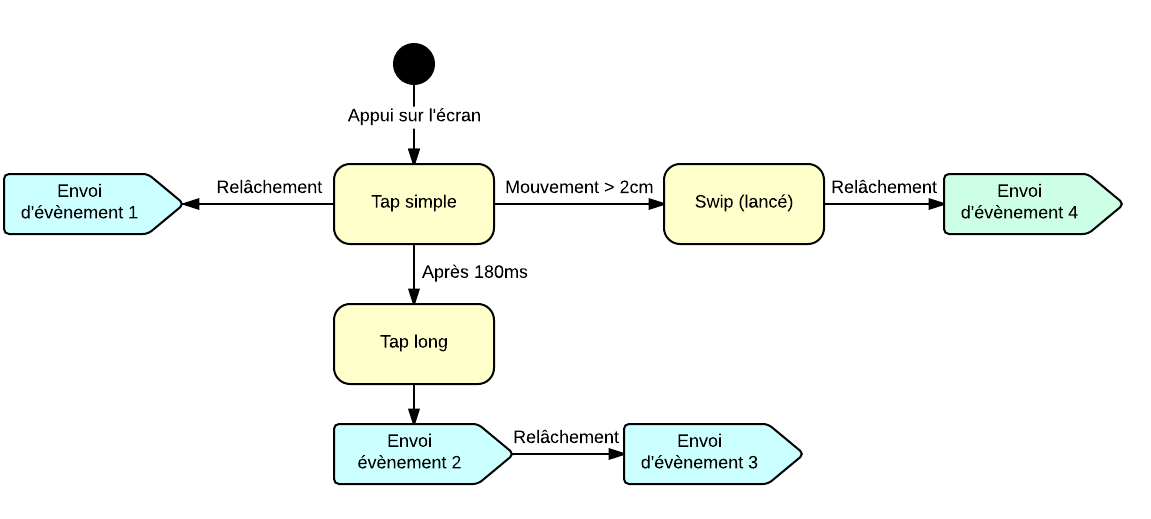
\includegraphics[scale=1]{./img/diagEtatTransition.png}}
\begin{center}
\textit{Diagramme d'états-transitions des évènements}
\end{center}

\paragraph{}
La gestion des évènements est délicate, dans le sens où elle se joue à quelques millisecondes prêt. Un temps d'attente trop long, et le joueur retrouve un décalage entre le moment où il appuie, et le moment où l'évènement est envoyé. Trop court, et le tap bref est interprété par un tap long, et le glissé n'a pas le temps de se faire. De même, une distance trop courte, et le moindre mouvement du doigt est interprété comme un lancement. Trop longue, et le risque qu'il soit interprété comme un évènement long, ou qu'un décalage se créé, apparaît. Ainsi de nombreux tests ont dû être effectués, nécessitant un mouvement infime des paramètres, et demandant à chaque fois de faire de nouveau une compilation, un transfert sur le téléphone et un test, puisque seule l'expérimentation permet de savoir si le réglage est bon.

\paragraph{Détection de la réussite}
Une fois les évènements convertis en numéros d'action, il faut vérifier si ces numéros sont en cohésion avec le niveau chargé. On ne compte que les échecs, et à la fin du niveau on soustrait le nombre total d'actions à réaliser par le nombre d'échecs pour obtenir le \% de réussite sur le niveau.
On ne met pas en place d'échelle de réussite comme on peut voir dans les autres jeux (mauvais, bon, parfait...). On considère que le joueur réussit ou rate un évènement.\\\\
Il y a deux types d'évènements à tester :
\begin{itemize}
\item Au moment où le joueur appuie, il faut vérifier que le numéro d'action tapé correspond au numéro d'action courant du niveau. On incrémente le nombre d'échecs si ça ne correspond pas.
\item Quand un évènement est passé, il vérifie si le joueur l'a réussi. Dans le cas où le joueur ne joue pas, il faut compter des erreurs.
\end{itemize}
\paragraph{}

La phase complexe est de déterminer quand un évènement est trop tôt ou trop tard. Un joueur ne frappera jamais pile au moment réel de l'évènement : Il faut mettre en place un système de tolérance.
\\\\
Après de multiples tests, nous avons conclu que le délais d'un quart de temps est suffisant comme négligence. C'est à dire que le joueur dispose d'un quart de temps complet pour réaliser une action demandée.
\\\\
On stocke dans une liste les numéros des ticks où le joueur a réussi. Quand le \textit{beateur} envoie un évènement, on regarde si le joueur a réussi le précédent. Sans quoi, on envoie un évènement \texttt{onFailure}.
\\\\
N'importe quel objet Unity peut se connecter à ce contrôleur. Ceci permet de construire le feedback visuel, en jouant par exemple une animation quand on reçoit un évènement \texttt{onFailure}.

\subsubsection{Résumé}

\noindent
\makebox[\textwidth]{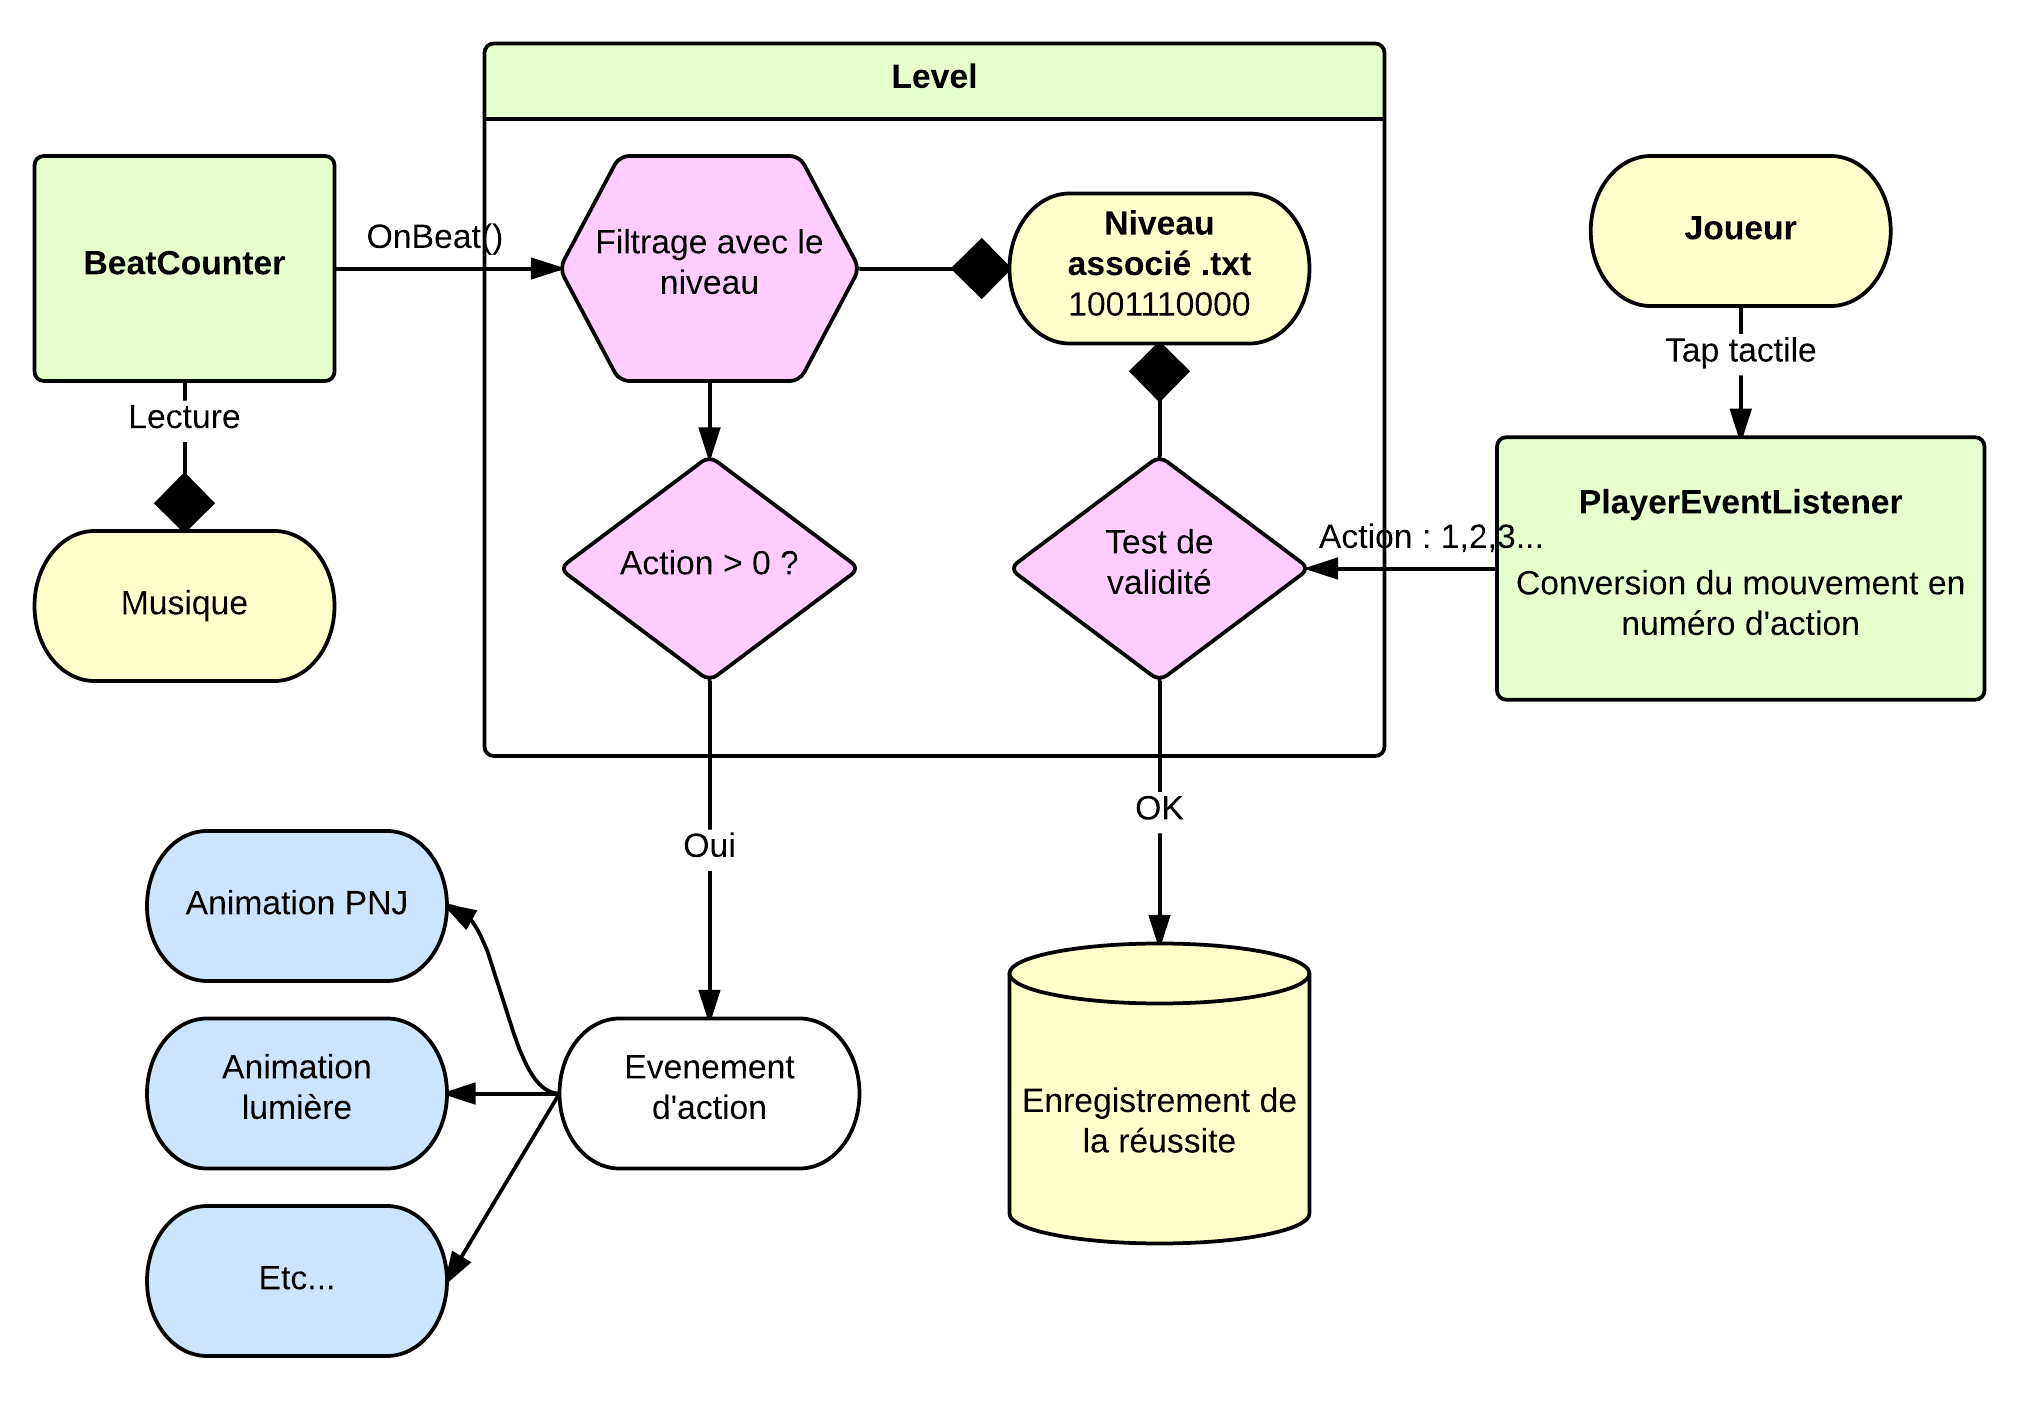
\includegraphics[scale=1]{./img/diagramme_moteur.png}}
\paragraph{}

Pour résumer le fonctionnement du moteur :
\begin{itemize}
\item Le \texttt{BeatCounter} lit la musique et envoie des évènements \texttt{OnBeat()} à chaque quart de temps.
\item Le \texttt{LevelScripted} filtre ces évènements en lisant le fichier, et envoie des évènements d'actions à tout les objets Unity qui l'écoutent
\item Quand le joueur tape sur l'écran, le \texttt{PlayerEventListener} convertit le mouvement en numéro d'action
\item Les actions du joueur sont validées par le \texttt{PlayerActions} qui enregistre si l'action correspond au fichier
\end{itemize}

\subsection{Outil de construction des niveaux}

Même si notre système de fichier est suffisamment clair pour être lu et modifié, il est difficile de construire des niveaux de façon aisée avec ce système. Il est beaucoup plus intéressant de créer les actions du niveau dans un logiciel de musique. Nous avons donc développé un outil de conversion pour générer ce genre de fichier à partir de fichiers MIDI.

\subsubsection{Structure d'un fichier midi}
Les spécifications du midi sont lourdes et complexes, elles ne seront pas détaillées ici, seules seront détaillées les informations importantes à notre convertisseur de niveau.

Un fichier midi est composé d'une suite de "chunks", eux mêmes composés d'évènements, il existe un certain nombre d'évènements différents, tels que le nom de la piste, le tempo, le nombre de pistes... Seuls un petit nombre de ces évènements nous sont utiles, ce sont ces évènements qui seront détaillés.\\
{\small \texttt{fichier midi = <header chunk> + <track chunk> [+ <track chunk> ...]}}\\\\
Un fichier midi commence par un \textit{header} formé de la manière suivante :\\
{\small \texttt{header chunk = "MThd" + <header length> + <format> + <n> + <division>}}\\

\begin{lstlisting}[language=Lisp]
;; lecture de l en-tete du fichier
(define (read-header in)
    (header (to-string (read-n-bytes in 4))
        (to-int (read-n-bytes in 4))
        (to-int (read-n-bytes in 2))
        (to-int (read-n-bytes in 2))
        (to-int (read-n-bytes in 2))))
\end{lstlisting}
{\small \texttt{track chunk = "MTrk" + <length> + <track event> [+ <track event> ...]}}\\\\
Un \textit{event} se présent sous la forme suivante :\\
{\small \texttt{track event = <delta time> + <midi event> | <meta event>}}\\\\
Les \textit{meta events} servent à donner des informations telles que le tempo, la division du tempo, ou la fin d'une \textit{track}.\\

\begin{lstlisting}[language=Lisp]
;; events utilises
(define time-signature-event '(255 88 4))
(define set-tempo-event '(255 81 3))
(define sequence-name-event '(255 3))
(define instrument-name-event '(255 4))
(define key-signature-event '(255 89 2))
(define smpte-offset-event '(255 84 5))
(define midi-channel-prefix-event '(255 32 1))
(define end-event '(255 47 0))
\end{lstlisting}

Les \textit{midi events} sont quand à eux des évènements directement en rapport avec la musique, le début ou la fin d'une note, ou encore le changement de canal.
{\small \texttt{midi event = <status byte> + <data byte> + <data byte>}}\\\\
Une fois lu, un fichier midi n'est rien d'autre qu'une suite d'octets, il est représenté dans notre programme comme valeurs de 0 à 255 : ‘(20 255 88 4 60 100 ...).

En parcourant le fichier, on peut reconnaître la suite d'octets "255 88 4", qui fait partie de nos évènement connus, on connaît également la taille de cet évènement, on sait donc que les 4 octets suivants formeront un \textit{event} de type "time signature".\\

\begin{lstlisting}[language=Lisp]
;;vrai si toutes les valeurs de l1 sont dans l2
(define (sublist? l1 l2)
    (andmap (lambda (i j)
        (= i j)) l1 (take l2 (length l1))))

;;vrai si les premiers octets de data
;;forment un event connu : e
(define (known-event? e data)
    (or (sublist? e data) (sublist? e (cdr data))))
\end{lstlisting}

Le delta time est codé avec une quantité à longueur variable. Le delta time n'est pas par rapport au début de la piste mais par rapport à l'évènement précédent.\\\\

\fbox{\parbox{11cm}
{\textbf{Note technique sur la quantité à longueur variable (\textit{variable-length quantity})}\\La vlq permet de représenter de manière compacte des quantités supérieures à un octet.

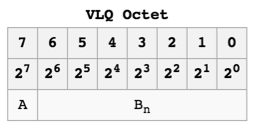
\includegraphics[scale=1]{./img/vlqOctet.png}\\
Si \texttt{A} est égal à 0, c'est que c'est le dernier octet de la quantité. Si c'est 1, un autre octet vlq suit.\\
\texttt{B} est un nombre de 7 bits, et \texttt{n} est la position de l'octet où \texttt{B0} est l’octet de poids faible.}
}\\\\

Certains éditeurs de fichiers midi utilisent une technique appelée le "running status" pour réduire la taille de leurs fichiers. Pour clairement comprendre son fonctionnement, une explication supplémentaire sur les \textit{midi events} s'impose.

Le \textit{status byte} a une valeur comprise entre 128 et 255, les \textit{data bytes} ont, quant à eux, une valeur comprise entre 0 et 127.

Le "running status" consiste à ne pas répéter le \textit{status byte} s'il est identique à l'évènement précédent. L'utilisation du "running status" est triviale à détecter et implémenter. En lisant le fichier, si l'octet lu est inférieur à 128 alors que l'on attendait un \textit{status byte}, c'est qu'il faut utiliser le dernier \textit{status byte} rencontré.

\subsubsection{Conversion en niveau}

En possession des ces informations, et avec la table des codes midi (voir annexe), convertir le fichier midi en niveau n'est alors plus qu'une succession de transformation de représentations. D'abord en \textit{chunks}, puis en \textit{tracks}, et enfin en \textit{events}, en filtrant les évènements inutiles à notre cas d'utilisation.\\
Une fois les évènements extraits du fichier midi, nous sommes en mesure de les convertir en actions pour notre jeu.

L'action 1 correspond à la note C, l'action 2 à la note C\#, et l'action 3 à la note D.
À chaque évènement avec le \textit{status byte} "début de note" (de l'octet 0x90 à l'octet 0x9F), l'action correspondant à la note de l'évènement est ajoutée au niveau. Ces actions sont séparées avec des zéros, eux donnés par le \textit{delta time}.\\

\begin{lstlisting}[language=Lisp]
;; transforme un evenement en donnees de niveau (0, 1, 2...)
;; division est le nombre de frames par secondes
;; delta-sum est la somme des delta depuis le dernier event utile
(define (event-to-level event division delta-sum)
    (let ([n (/ (+ delta-sum (vlq->int (midi-event-delta event))) (/ division 4))])
    ; n est le nombre de temps ou rien ne se passe (0)
    ; midi-event-arg1 est la note
    ; notes est la hashmap ou sont faites les correspondances
    (append (make-list n 0) `(,(hash-ref notes (midi-event-arg1 event) #\?)))))
\end{lstlisting}


\subsubsection{Mise en pratique}
On utilise dans cet exemple le logiciel Logic Pro X sous Mac OS X. N'importe quel autre séquenceur gérant les fichiers MIDI peut être utilisé.\\

On importe la musique sur une piste, et on fixe le tempo de celle-ci.\\
\begin{center}
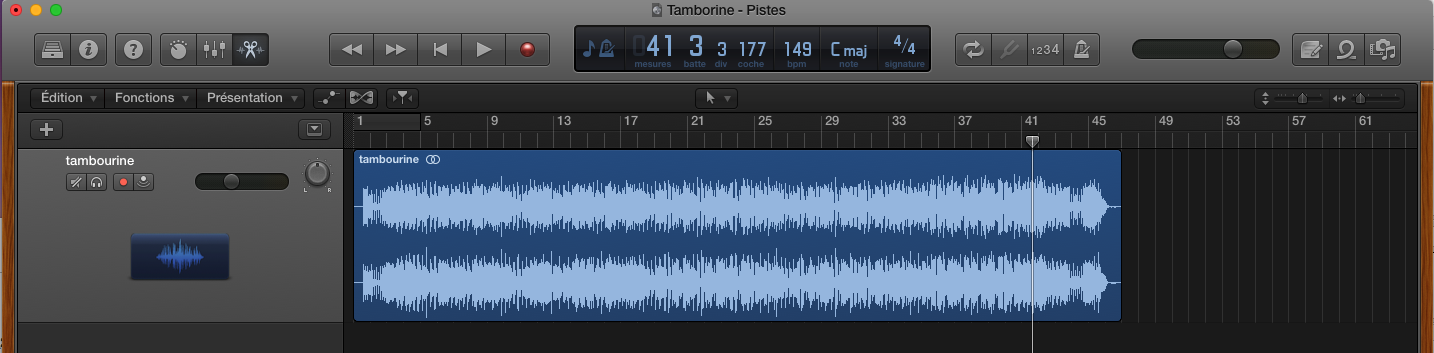
\includegraphics[width=11cm]{./img/logic_sound.png}\\
\end{center}

On ajoute sur une seconde piste vide un instrument qui représente le niveau à créer, sur laquelle on va ajouter les actions.\\
\begin{center}
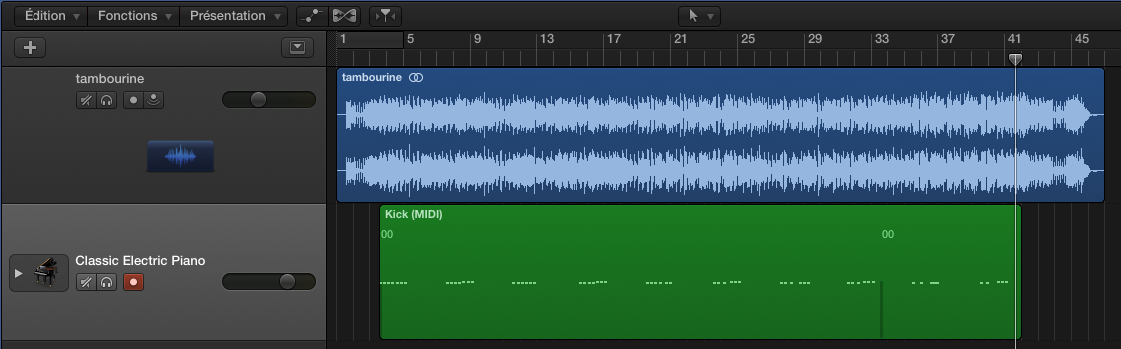
\includegraphics[width=11cm]{./img/logic_midi.png}\\
\end{center}

On pose ensuite les notes qui représentent les actions sur cette piste, puis on écoute le tout en temps réel pour superposer proprement chacune des actions sur la musique. On utilise des notes différentes pour chaque type d'action. Ici le DO pour une action 1, le DO\# pour une action 2, etc.\\
\begin{center}
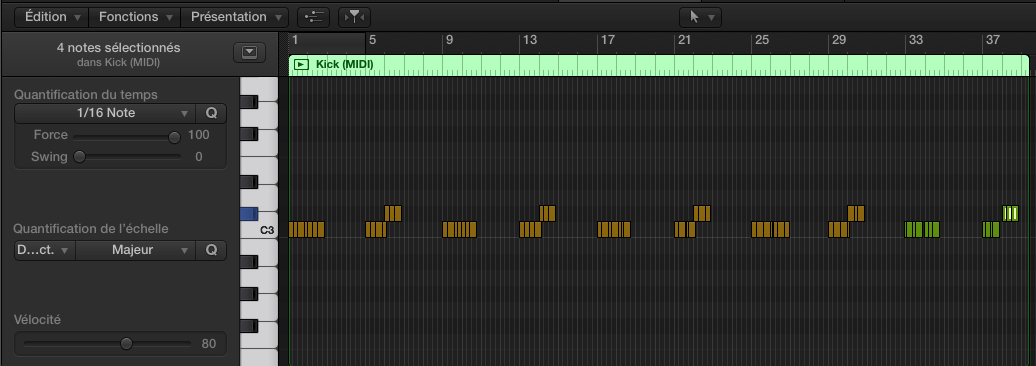
\includegraphics[width=11cm]{./img/logic_edit.png}\\
\end{center}

Une fois le niveau construit, il ne reste plus qu'à exporter la piste au format .midi, et de le passer au convertisseur pour obtenir le niveau au format .txt.\\
\begin{center}
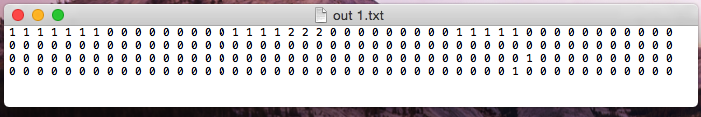
\includegraphics[width=11cm]{./img/logic_export.png}\\
\end{center}

\subsection{Le gameplay}

Expérience utilisateur, graphismes, feedback, analyse...








\subsection{Tests}
\subsubsection{Pendant le développement}
\subsubsection{Sur la version pre-release}